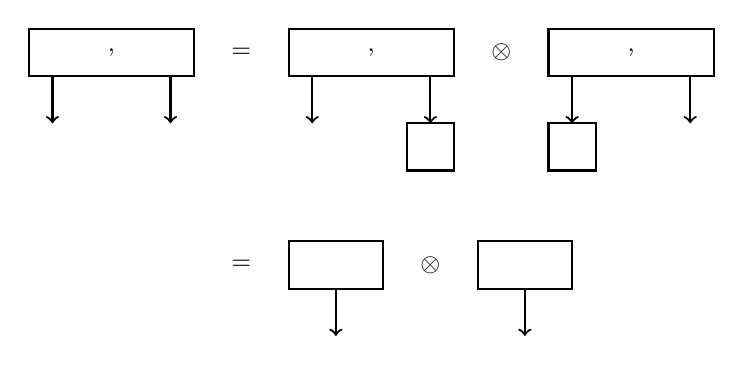
\begin{tikzpicture}[scale=0.3,thick] % , baseline = -3.5pt


\draw (0,1) rectangle (7,-1);
\node[anchor=center] (text) at (3.5,0) {\small $\probof{\exrandom,\secexrandom}$};
\draw[->] (1,-1) -- (1,-3) node[midway, left] {\tiny $\exrandom$};
\draw[->] (6,-1) -- (6,-3) node[midway, left] {\tiny $\secexrandom$};

\node[anchor=center] (text) at (9,0) {\small ${=}$};


\begin{scope}[shift={(11,0)}]

\draw (0,1) rectangle (7,-1);
\node[anchor=center] (text) at (3.5,0) {\small $\probof{\exrandom,\secexrandom}$};
\draw[->] (1,-1) -- (1,-3) node[midway, left] {\tiny $\exrandom$};
\draw[->] (6,-1) -- (6,-3) node[midway, left] {\tiny $\secexrandom$};
\draw (5,-3) rectangle (7,-5);
\node[anchor=center] (text) at (6,-4) {\small $\ones$};

\end{scope}

\node[anchor=center] (text) at (20,0) {\small $\otimes$};



\begin{scope}[shift={(22,0)}]

\draw (0,1) rectangle (7,-1);
\node[anchor=center] (text) at (3.5,0) {\small $\probof{\exrandom,\secexrandom}$};
\draw[->] (1,-1) -- (1,-3) node[midway, left] {\tiny $\exrandom$};
\draw (0,-3) rectangle (2,-5);
\node[anchor=center] (text) at (1,-4) {\small $\ones$};
\draw[->] (6,-1) -- (6,-3) node[midway, left] {\tiny $\secexrandom$};

\end{scope}



\node[anchor=center] (text) at (9,-9) {\small ${=}$};


\begin{scope}[shift={(11,-9)}]

\draw (0,1) rectangle (4,-1);
\node[anchor=center] (text) at (2,0) {\small $\probof{\exrandom}$};
\draw[->] (2,-1) -- (2,-3) node[midway, left] {\tiny $\exrandom$};

\node[anchor=center] (text) at (6,0) {\small $\otimes$};

\draw (8,1) rectangle (12,-1);
\node[anchor=center] (text) at (10,0) {\small $\probof{\secexrandom}$};
\draw[->] (10,-1) -- (10,-3) node[midway, left] {\tiny $\secexrandom$};


\end{scope}

%\node[anchor=center] (text) at (46,-3) {\small ${.}$};

\end{tikzpicture} 